\section{Chomsky Hierarchy}
\scriptsize{Notational Concentions}\\ {\tiny T: lower case Latin letters(e.g. a,b,c,x,y,z) \\
NT: upper case Latin letters(e.g. A,B,C,X,Y,Z) \\
strings of T and NT symbols: lower case greek letters(e.g. $\alpha, \beta, \gamma$ }\\
\scriptsize{Regular lanugages/finite state grammars/type 3}\\ {\tiny X -> x, 
X -> xY\\
(beware: different usages: X -> YZ where Y $\neq$ Z)\\
examples: set of strings following the pattern x**ny**m; set of strings such that number of 'a's is a multiple of 4; set of natural numbers that leave a remainder of 3 when divided by 5...\\
If...then...; either...or...; the..., is...; in natural languages cannot be generated by regular grammars\\
Limitations: for certain constructions, e.g. of the anbn typle, they will also generate ungrammatical sentences; since at least 1 terminal symbol has to be produced in every rewrite, no higher level patterns (phrase structures) can be captured
}\\
\scriptsize{Context-free languages/type 2}\\ 
{\tiny X -> $\beta$, only allow 1 single non-terminal on the left hand side, but an arbitrary string of terminals and non-terminals on the right hand side.\\
Examples of generated languages: \\
mirror langauge abba, abccba, acbddcba...\\
palidrome language: aba, bab, abba...\\
languages with form x**ny**mz**mw**n\\
Natural language not context-free? (Swiss German ambncmdn, Bambara)\\
Summary: more powerful than regular grammars; taken its binarized version, boils down to having 1 additional rule pattern compared to regular grammars X -> YZ (Y=Z allowed)
}\\
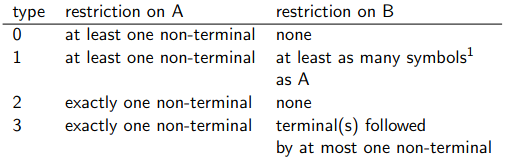
\includegraphics[scale=0.25]{chomsky.png}\\
\scriptsize{Context-sensitive languages/type 1}\\ {\tiny $\varphi_1 X \varphi_2 \to \varphi_1 \beta \varphi_2$, X is a single non-terminal X, the context may be null\\
alternative version: $\alpha \to \beta$, with $\beta$ at least as long as $\alpha$\\
example: copy language aa, abab, abcabc...\\
languages with strings of form x**ny**nz**n\\
set of all prime numbers (where each number represented by a string of length I(x))\\
assumption that natural languages are at least mildly context-sensitive
}\\
\scriptsize{Recursively enumerable languages/type 0}\\{\tiny $\alpha \to \beta$
}\\
\scriptsize{Classical hierarchy}\\ {\tiny regular (a**nb**m) finite-state automaton \\
context-free (a**nb**n) push-down automaton\\
context-sensitive (a**2**n) linear-bounded automaton\\
type-0 (a**n) Turing machine
}\\
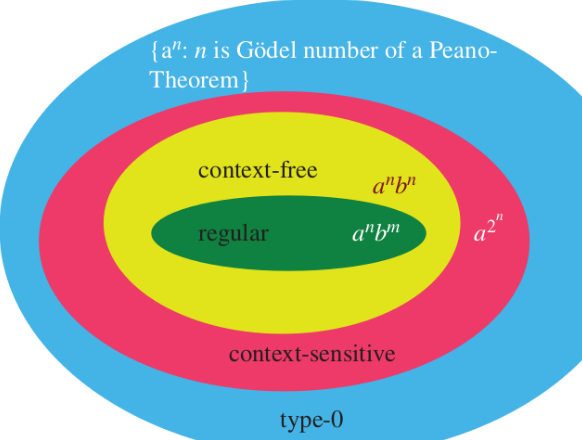
\includegraphics[scale=0.15]{chomsky-hierarchy.png}